
%%letter, article, report, book
\documentclass[12pt]{article}
\usepackage[margin=1in]{geometry}
\usepackage{setspace}
\usepackage{harvard}
\usepackage{graphicx}
\usepackage{float}

\begin{document}

\title{C.C.A.S.A. \\
	Car Concentration And Security Assistant}
\author{Bracco Filippo e Di Vece Chiara}
\maketitle

	
	\begin{abstract}
		
		\begin{center}
			Stanchezza, nervosismo, distrazione e sonnolenza sono le cause di oltre il 66\% degli incidenti. Questi dati allarmanti ci hanno indotto a voler realizzare un dispositivo che possa evitare incidenti di questa natura verificando oggettivamente che il conducente sia sempre concentrato sulla strada. Lo scopo del prototipo \`{e} quello di rilevare particolari condizioni non compatibili con una guida sicura attraverso il rilevamento dei tratti del viso, e in particolar modo degli occhi, accertandosi che lo sguardo sia rivolto verso la strada mentre il veicolo \`{e} in movimento. In seguito risponder\`{a} adeguatamente per richiamare all'attenzione il guidatore con avvisi acustici e visivi. Coscienti dei limiti della nostra idea e di quelli delle nostre capacit\`{a}, intendiamo realizzare un prototipo semplificato che svolga le funzioni appena elencate e che, magari, possa essere implementato per poter essere realmente installato in un'autovettura per salvare il maggior numero possibile di vite.
			
		\end{center}
		
		
		\begin{center}
			
			\textbf{Key words}: Face detection, gesture identification, sicurezza alla guida
			
		\end{center}
		
		
	\end{abstract}
	
	\pagebreak
	
	\section{What we planned...}
	
	\subsection{Pre-accensione}
	
	Inizialmente il quadro dell'automobile \`{e} spento, così come il diplay (sostituito da un riquadro nero) e si attende la pressione del tasto 's' per avviare il programma.
	
		\begin{figure}
\centering
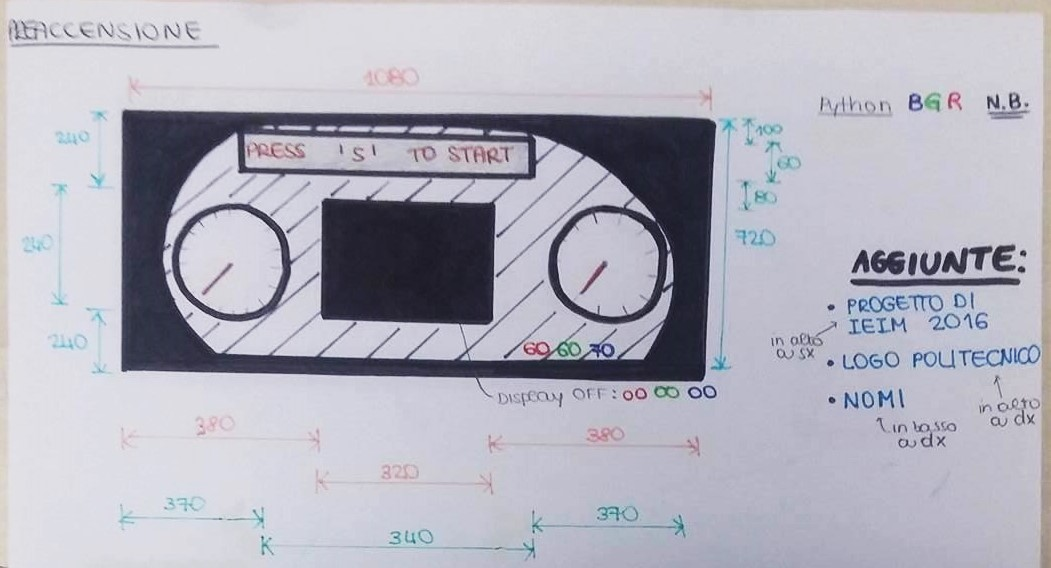
\includegraphics[width=0.7\linewidth]{../Assets/Img/1.jpg}
\caption{}
\label{fig:1}
\end{figure}


		
	\subsection{Accensione}
	
	Dopo la pressione del tasto 's' il quadro si accende e il suo colore passa da grigio a verde e contemporaneamente, il riquadro nero centrale, \`{e} sostituito dal display che mostra ciò che vienen acquisito al momento dalla webcam. A questo punto vengono valutate le condizioni di guida, inizialmente considerate sicure.
	
	\subsubsection{Guida sicura}
	
	Se la guida \`{e} ritenuta sicura comparir\`{a} il riquadro verde visibile in alto al centro con la scritta "GUIDA SICURA!"; verranno rilevati sia il volto che gli occhi del guidatore ed essi saranno riquadrati in verde.
	
		\begin{figure}[H]
			\centering
			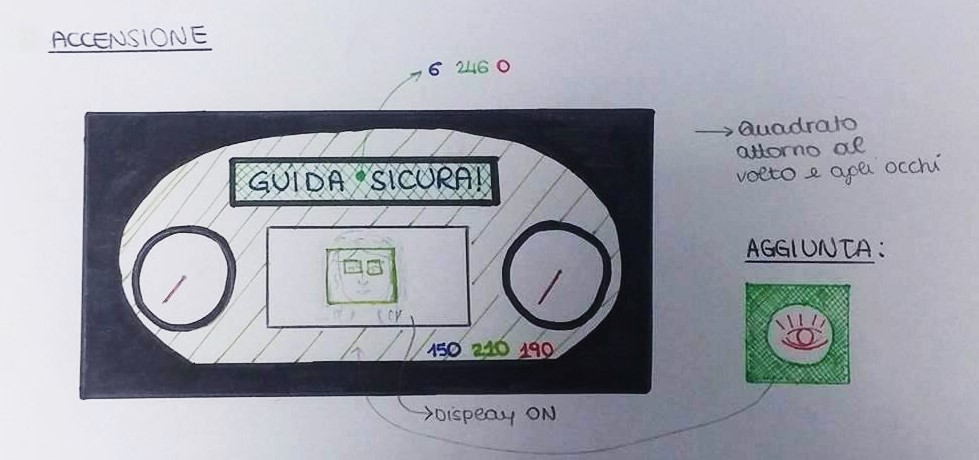
\includegraphics[width=1.0\linewidth]{../Assets/Img/2.jpg}
			\caption{Guida sicura}
			\label{fig:2}
		\end{figure}

	
	\subsubsection{Distrazione}
	
	Se il contucente non ha il volto rivolto verso la strada non verranno rilevati n\`{e} il volto n\`{e} gli occhi; in seguito a ci\`{o} comparir\`{a} un riquadro giallo con la scritta "DISTRAZIONE!" a cui sar\`{a} accompagnato un avviso acustico.
	
		\begin{figure}[H]
			\centering
			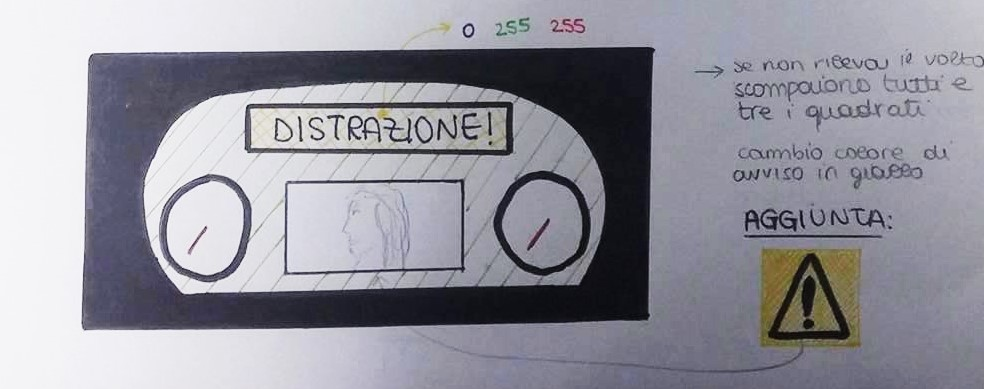
\includegraphics[width=1.0\linewidth]{../Assets/Img/3.jpg}
			\caption{Guida distratta}
			\label{fig:3}
		\end{figure}

	
	\subsubsection{Guida pericolosa}
	
	Se il guidatore chiude gli occhi perchè assonnato gli occhi non verranno pi\`{u} rilevati e comparir\`{a} un riquadro rosso con la scritta "PERICOLO!" a cui sar\`{a} accompagnato un avviso acustico pi\`{u} intenso.
	
		\begin{figure}[H]
			\centering
			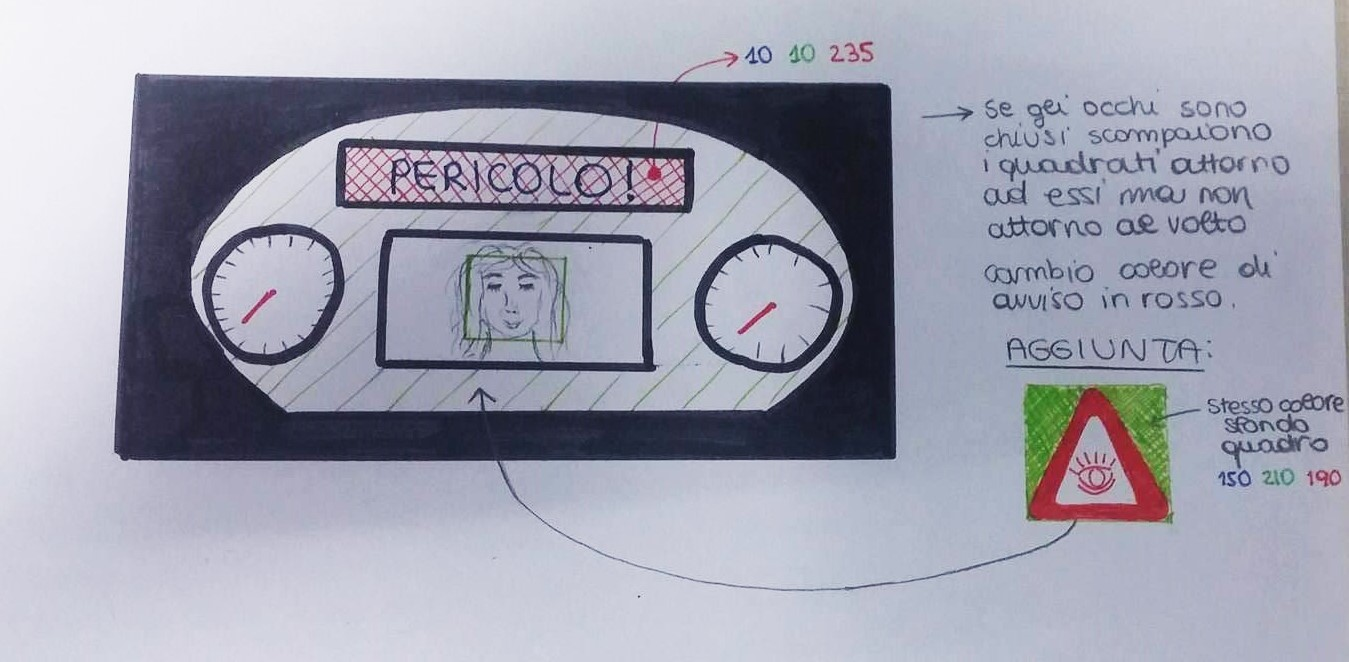
\includegraphics[width=1.0\linewidth]{../Assets/Img/4.jpg}
			\caption{Guida pericolosa}
			\label{fig:4}
		\end{figure}

		
	\section{...what we did!}	
	
	\subsection{Guida sicura}
	
		\begin{figure}[H]
			\centering
			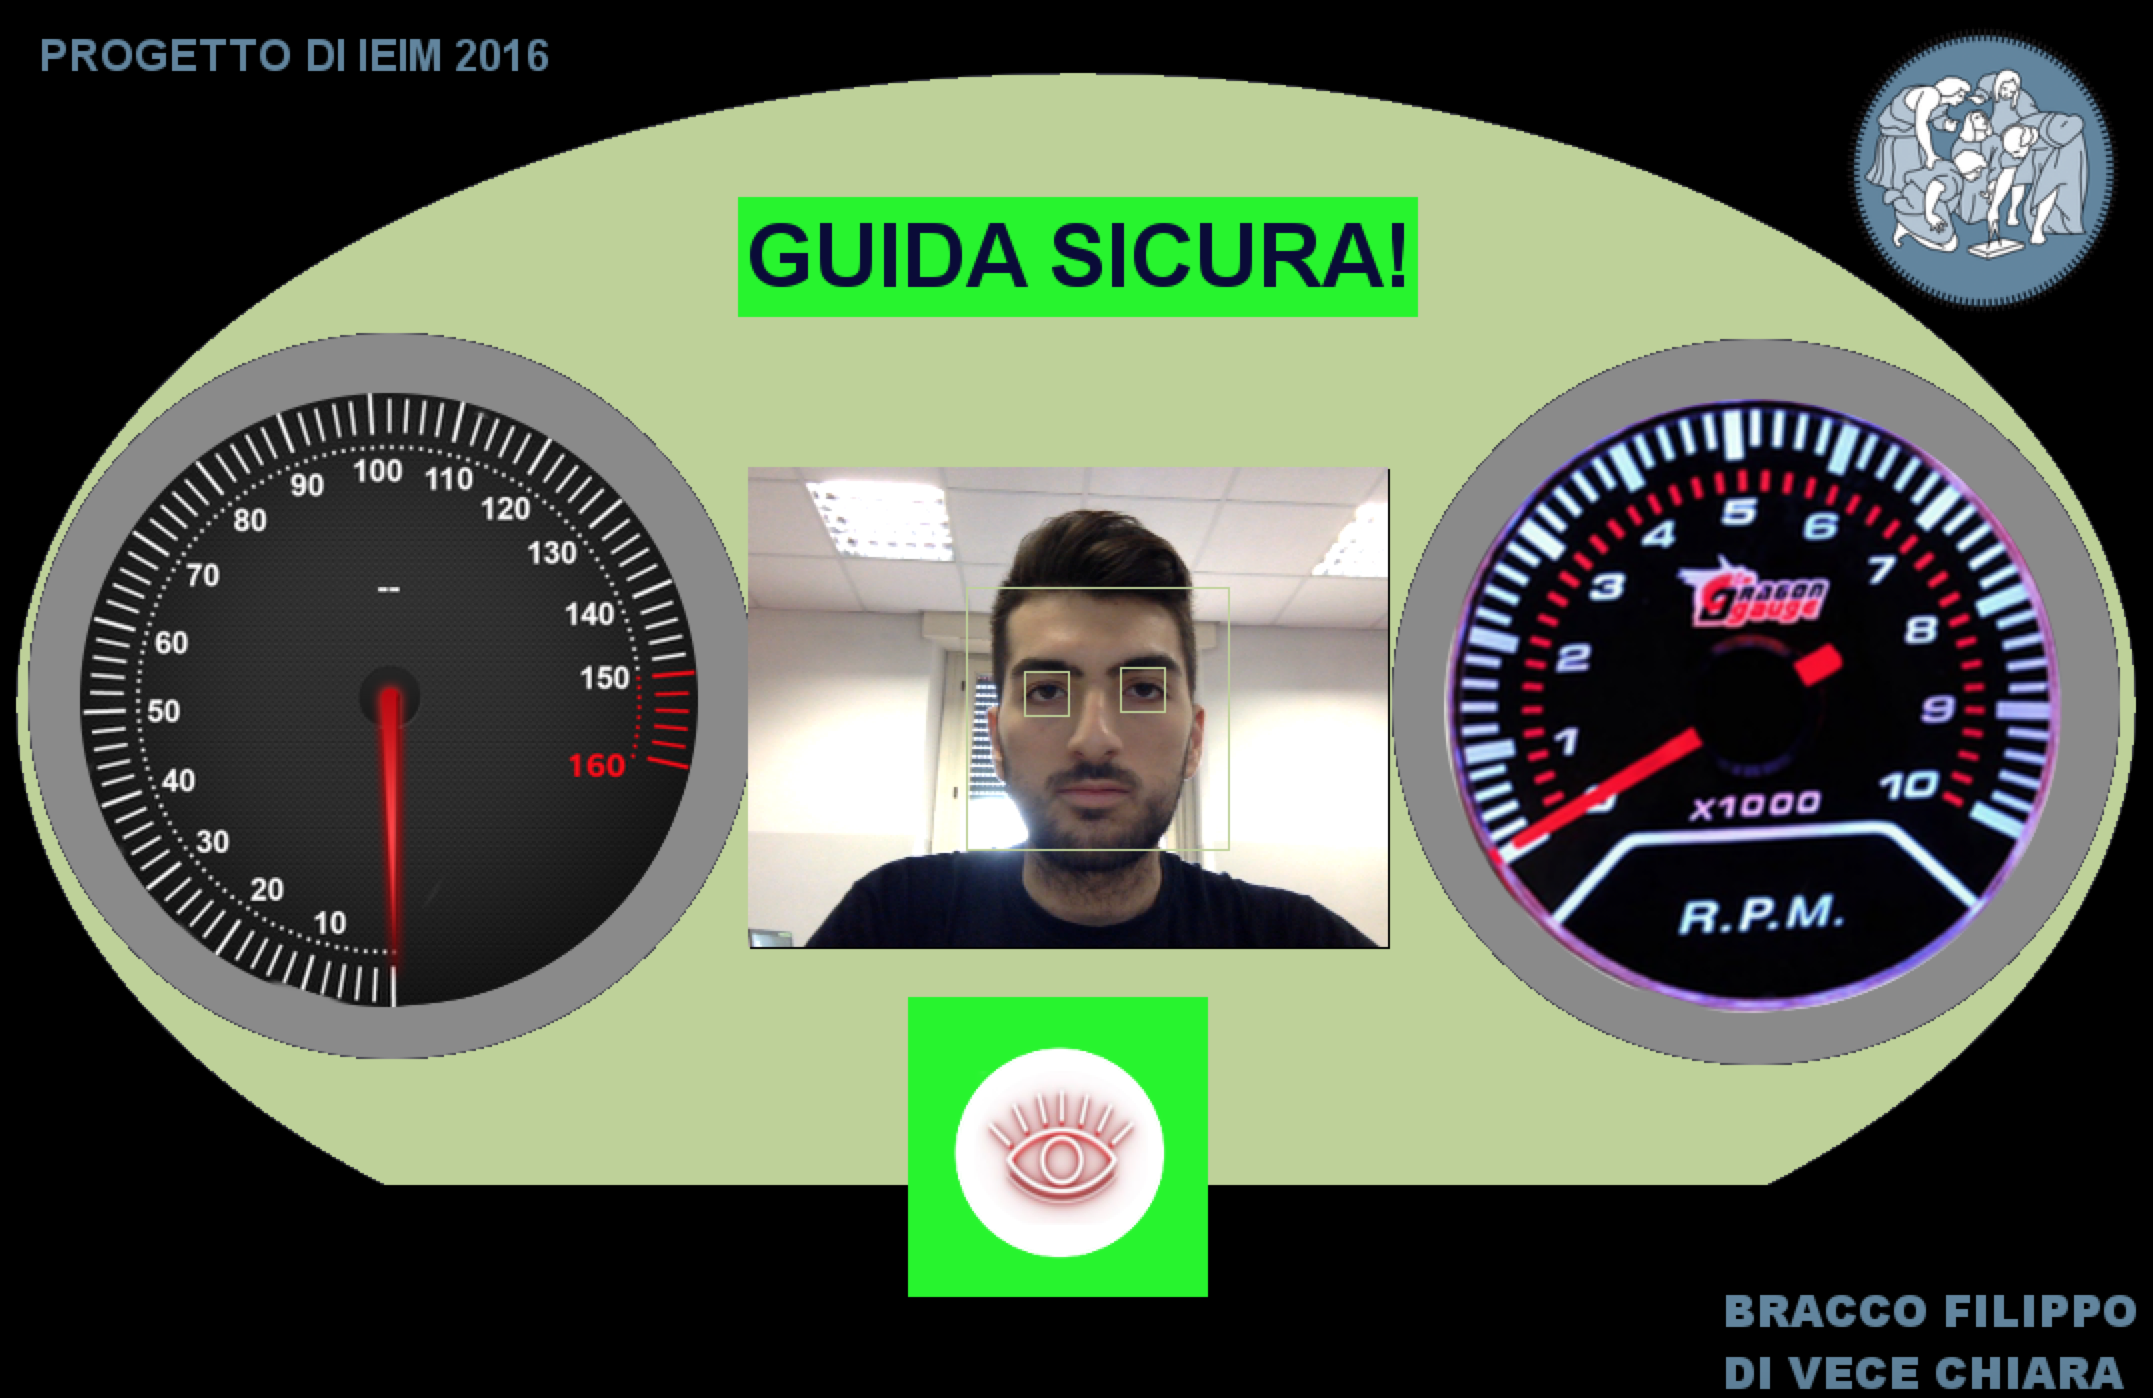
\includegraphics[width=0.8\linewidth]{../Assets/Img/guida_sicura_tex.png}
			\caption{Guida sicura}
			\label{fig:guidasicura}
		\end{figure}

		
	\subsection{Distrazione}
	
		\begin{figure}[H]
			\centering
			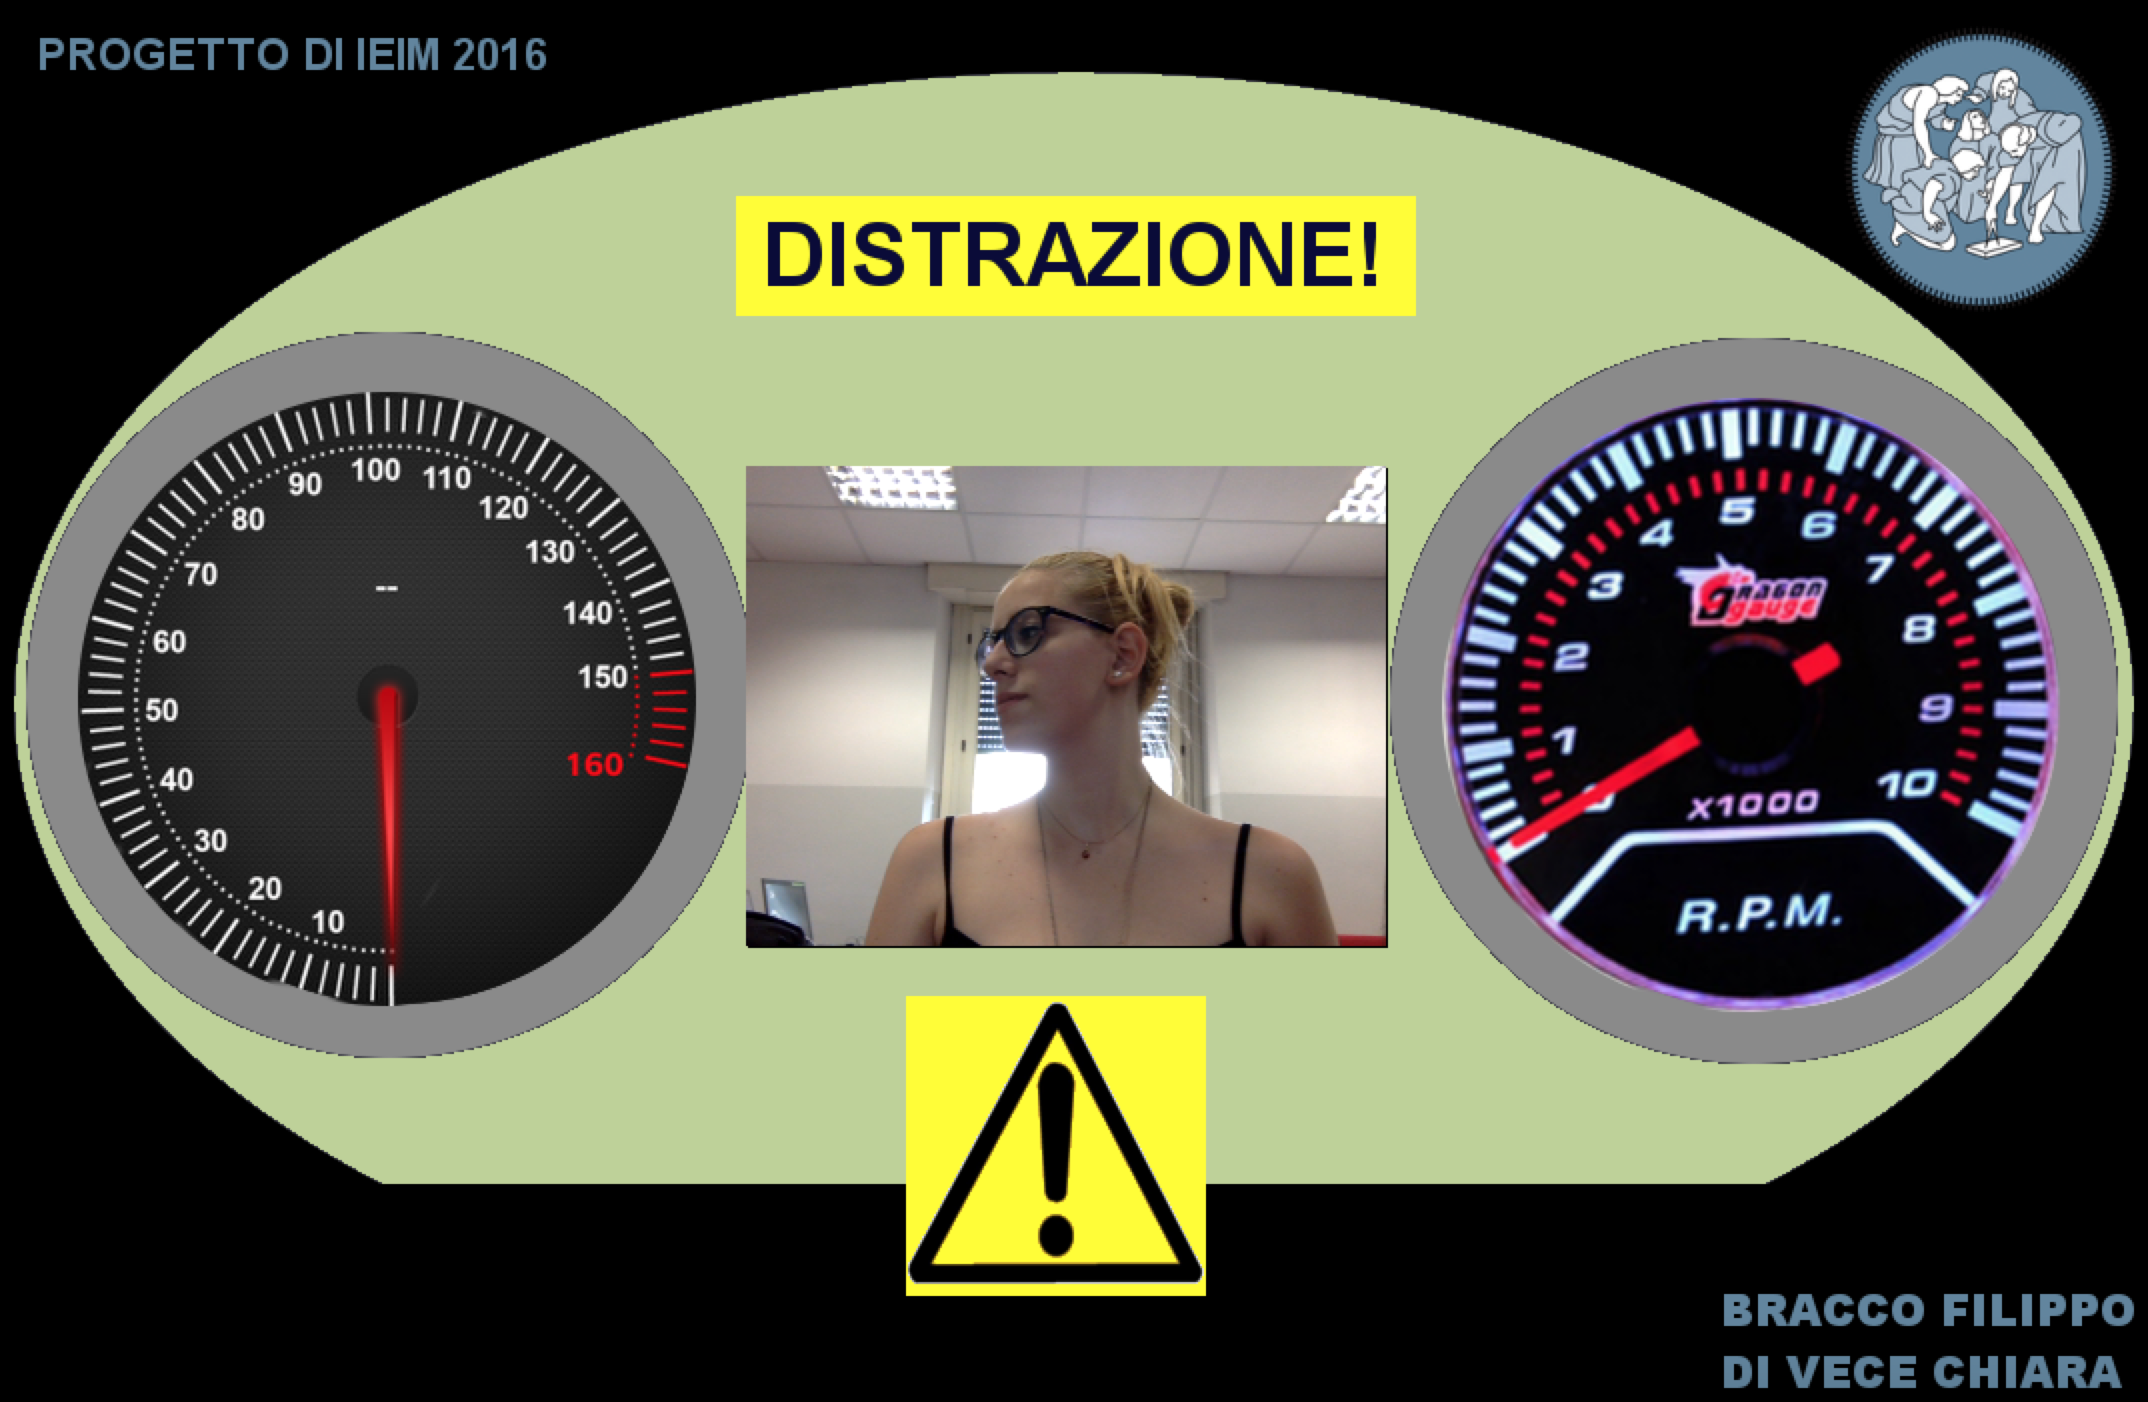
\includegraphics[width=0.8\linewidth]{../Assets/Img/guida_distratta_tex.png}
			\caption{Guida distratta}
			\label{fig:guidadistratta}
		\end{figure}


	\subsection{Guida pericolosa}
	
		\begin{figure}[H]
			\centering
			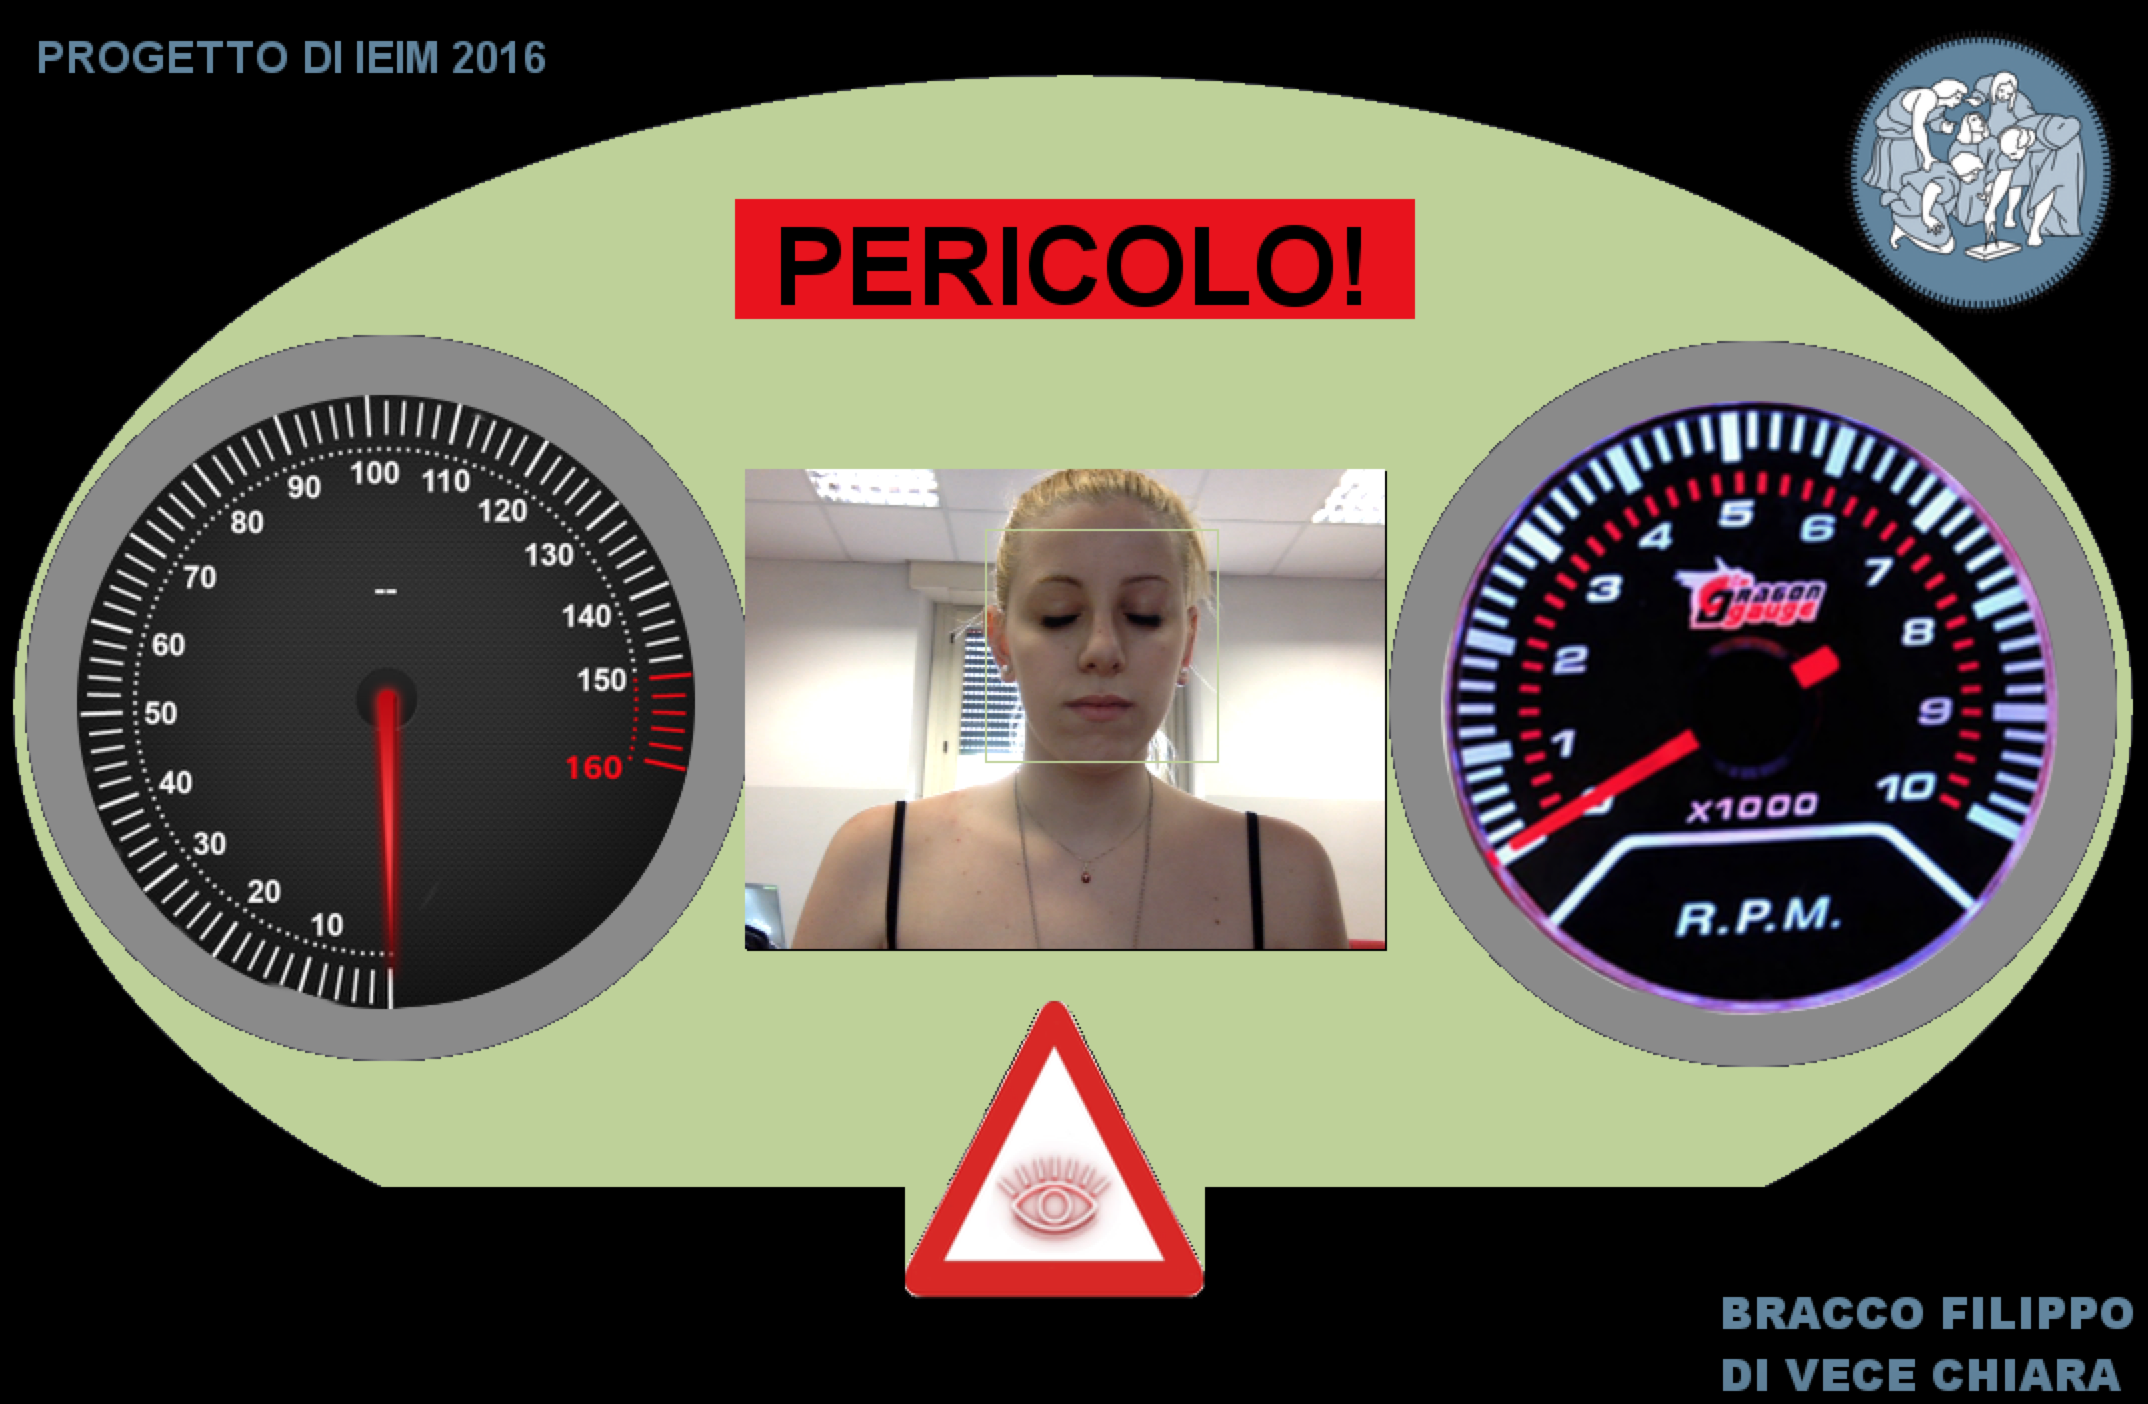
\includegraphics[width=0.8\linewidth]{../Assets/Img/guida_pericolosa_tex.png}
			\caption{Guida pericolosa}
			\label{fig:guidapericolosa}
		\end{figure}


\end{document}


